%% LyX 2.3.0 created this file.  For more info, see http://www.lyx.org/.
%% Do not edit unless you really know what you are doing.
\documentclass[english]{article}
\usepackage[T1]{fontenc}
\usepackage[latin9]{inputenc}
\usepackage{geometry}
\geometry{verbose,tmargin=3cm,bmargin=3cm,lmargin=3cm,rmargin=3cm}
\setlength{\parskip}{6pt}
\setlength{\parindent}{0pt}
\usepackage{verbatim}
\usepackage{amsmath}
\usepackage{amssymb}
\usepackage{graphicx}
\usepackage[authoryear]{natbib}

\makeatletter

%%%%%%%%%%%%%%%%%%%%%%%%%%%%%% LyX specific LaTeX commands.
%% A simple dot to overcome graphicx limitations
\newcommand{\lyxdot}{.}


%%%%%%%%%%%%%%%%%%%%%%%%%%%%%% Textclass specific LaTeX commands.
\newenvironment{lyxcode}
	{\par\begin{list}{}{
		\setlength{\rightmargin}{\leftmargin}
		\setlength{\listparindent}{0pt}% needed for AMS classes
		\raggedright
		\setlength{\itemsep}{0pt}
		\setlength{\parsep}{0pt}
		\normalfont\ttfamily}%
	 \item[]}
	{\end{list}}

%%%%%%%%%%%%%%%%%%%%%%%%%%%%%% User specified LaTeX commands.
\sloppy
%\setlength{\parskip}{6pt}

\@ifundefined{showcaptionsetup}{}{%
 \PassOptionsToPackage{caption=false}{subfig}}
\usepackage{subfig}
\makeatother

\usepackage{babel}
\begin{document}
\global\long\def\taxonomy{\mbox{\ensuremath{\mathbb{T}}}}

\global\long\def\prunedTaxonomy{\taxonomy_{P}}

\global\long\def\phyloinputs{\mathcal{T}}

\global\long\def\expandedPhylo{\phyloinputs_{E}}

\global\long\def\summaryTree{\mathbb{S}}

\global\long\def\prunedSummary{\summaryTree_{P}}

\global\long\def\collections{\mathcal{C}}


\title{\texttt{Taxonomic supertree construction with}\texttt{\emph{ Incertae
sedis}}\texttt{ taxa}}
\maketitle

\section{Introduction}

Supertree methods combine a collection of input trees with different
taxon sets into a single tree on the combined taxon set. While such
methods are usually applied to leaf-labeled phylogenies that have
been estimated from DNA sequence data, we seek to include taxonomic
information also. Taxonomies can provide a comprehensive coverage
of known taxa that inferred phylogenies cannot. Additionally, taxonomies
can provide taxonomic names, which are needed to align input phylogenies
to each other, and to allow references to existing groups.

We thus require that one of the input trees is a taxonomy tree. The
taxonomy has a number of features not found in the input phylogenies.
While the input trees need not cover the entire taxon set, we require
the taxonomy to be comprehensive. The taxonomy also has labels for
internal nodes, whereas input phylogenies only have labels for leaf
nodes. We refer to labels of taxonomy nodes as ``taxon names'',
and require that taxon names and taxonomy nodes have a one-to-one
correspondence. The taxonomy may also contain out-degree 1 nodes.
These nodes correspond to monotypic taxa which contain a single child
of lower taxonomic rank.

In practice, taxonomies may also contain nodes with uncertain placement.
These nodes are often labelled ``\emph{incertae sedis}'', which
means ``uncertain seat'' in Latin. The common interpretation of
such taxa is that they may not be moved further towards the root,
but may be moved into their sibling taxa. For example, a genus with
a sibling that is a family may be annotated as``\emph{incertae familia}'',
indicating that it is unclear which family the genus should be placed
in. \emph{Incertae sedis} taxa frequently occur when a specimen is
identified up to a given taxonomic level, but no further. Extinct
taxa are often \emph{incertae sedis}.

The Open Tree of Life project seeks to build a comprehensive supertree
covering all of life. The approach is to combine information in published
phylogenies with a comprehensive taxonomy that supplies taxon names
\citep{redelings2017supertree}. We describe an extension to this
supertree method so that we can resolve taxonomic uncertainty by using
published phylogenies to place \emph{incertae sedis} taxa. We describe
an updated semantics for conflict between phylogeny edges and taxonomy
edges and an updated semantics for assigning taxonomy names to nodes
in the synthetic tree. 

Our approach to \emph{incertae sedis} taxa enables us to use published
phylogenies to update the taxonomy by extending taxonomic groups to
include \emph{incertae sedis} taxa placed within them. The ability
to update the taxonomy is important, since the placement of \emph{incertae
sedis} taxa creates artificial conflicts with a non-updated taxonomy.
Thus, the ability to correctly assess compatibility with the taxonomy
when the taxonomy contains \emph{incertae sedis taxa} allows us to
include thousands of new taxa that were previously filtered out to
avoid conflict. It also enables us to include extinct taxa, since
many of these taxa are \emph{incertae sedis}. This makes substantial
progress towards our goal of completely representation of taxa.

\subsection{Background}

\paragraph{Terminology}

We briefly describe the supertree algorithm proposed in \citet{redelings2017supertree}.
This supertree algorithm takes as input a ranked list $\phyloinputs=\left\{ T_{1},\ldots,T_{n}\right\} $
of rooted input phylogenies and a single rooted taxonomy tree $\taxonomy$.
Each node in the taxonomy tree is associated with a taxon name in
the set of taxon names $\mathcal{N}$, and each taxon name is corresponds
to only one node of the taxonomy tree. We use \emph{$\mathcal{L}$
}to indicate taxon names corresponding to leaf nodes of the taxonomy
tree. Correspondence between the input trees and the taxonomy is established
by annotating leaf nodes of each input tree with taxon names. For
purposes of conflict resolution, the taxonomy tree is ranked below
all of the input trees. 

In this manuscript we extend this framework by adding a set $\mathcal{U}\subseteq\mathcal{N}$
of labels that have the \emph{incertae sedis }property. The extended
taxonomy then consists of the taxonomy tree $\taxonomy$, the labels
$\mathcal{N}$, and set $\mathcal{U}$ of \emph{incertae sedis }taxa.

\paragraph{Exemplification}

While the taxonomy is comprehensive and contains all taxa, input phylogenies
only have labels on their leaf nodes, and generally include a small
fraction of the total number of taxa. Furthermore, taxa in input trees
may correspond to higher taxa on the taxonomy tree, and multiple tips
may be labeled with the same taxon name. \citet{redelings2017supertree}
described a method called 'exemplification' that reduces this problem
to a simpler form where all taxon names of input trees (i) correspond
to leaf taxa and (ii) occur only once in an input tree. For the purposes
of this paper, we therefore assume that this is the case.

\paragraph{Problem decomposition}

Given the exemplified input trees and taxonomy, the supertree algorithm
first divides the supertree problem into independent pieces, solves
the problem on these pieces, and then glues the pieces back together.
This is made possible by the assumption that any taxonomy edges that
are not contested by any of the input trees can be assumed to occur
in the supertree. We may then solve separately for what happens on
each side of such an uncontested edge. When the uncontested edge is
attached to the solution below the edge and the solution above the
edge, the complete solution is then obtained.

\paragraph{Splits-based synthesis method}

Supertrees for each subproblem are obtained by greedily constructing
a set of rooted splits $\mathcal{C}$ that are jointly consistent
and correspond to branches of the input trees. We construct an ordered
list of splits $S(T_{i})$ by walking the branches of each tree $T_{i}$
in post-order and appending the corresponding splits to the list.
These lists are combined to form the list $\Sigma=S(T_{1})+S(T_{2})+\ldots+S(T_{n})+S(\mathbb{T})$,
where '$+$' denotes concatenation. The set $C$ is initialized to
the empty set, and we then iteratively consider each split in the
list $\Sigma$ and insert it into $C$ if the resulting set remains
jointly compatible. The BUILD algorithm is used both to check compatibility,
and to construct a compatible tree from the final set $C$.


\section{\label{sec:Semantics-of-incertae}Semantics of \emph{incertae sedis}
taxa}

 We seek a semantics for supertrees with \emph{incertae sedis }taxa
that satisfy the following properties:
\begin{enumerate}
\item An incertae sedis node may intrude into its siblings and their descendants.
\item Two incertae sedis siblings may not be interdigitated.
\item Any placement $T\to T^{*}$ of a tree $T$ with incertae sedis taxa
is also accessible from a tree $T^{\prime}$ that is created from
$T$ by taking a taxon, attaching it to an ancestor, and marking it
\emph{incertae sedis}.
\item The semantics of an \emph{incertae sedis} node does not depend on
assigned ranks, but only on the tree.
\item Semantics is based on deriving a split for each branch of the tree.
\end{enumerate}
Here we focus on a split-based semantics instead of a semantics based
on apply of a series of edit operations to the tree. The split-based
semantics allows us to seek trees that are simultaneously consistent
with a set of split-constraints. The use of a split-based semantics
does impose some limitations. These come primarily because in the
edit-based semantics, after we place an \emph{incertae sedis} taxon,
it is no loner \emph{incertae sedis}, whereas with the split-based
semantics taxa are either always \emph{incertae sedis} or never \emph{incertae
sedis}.

This has an effect, for example, when we consider two incertae sedis
siblings $A$ and $B$. If we can place $A$ within $B$, and $B$
within $A$, then a split-based semantics allows us to freely inter-digitate
$A$ and $B$. If we do not want to allow $A$ and $B$ to be inter-digitated,
then we cannot both $A$ within $B$ and $B$ within $A$. In addition,
we can imagine that a family $A$ is incertae sedis within a kingdom.
In an edit-based semantics, we could place $A$ as a sibling to a
genus $B$, mark $A$ as non-\emph{incertae-sedis}, and then place
$B$ within $A$. In a split-based semantics, we must disallow either
$B$ within $A$ or $A$ within $B$ if we want to disallow interdigitation.

As a result of this, we cannot satisfy all five of these criteria.
Thus, we describe two alternative split-based semantics. The non-interdigitation
semantics gets \# (1,2,4,5), and the interdigitation semantics gets
(1,3,4,5). This makes the point that each semantics results from different
choices about which criteria to satisfy.

\subsection{Split-based semantics for \emph{incertae sedis} taxa}

In order to apply supertree methods to rooted trees with \emph{incertae
sedis} taxa, we first propose a semantics of \emph{incertae sedis
}in terms of rooted splits. We define rooted splits by noting that
each edge of a tree divides the tip taxa $\mathcal{L}$ into two groups:
the include set $\mathcal{I}(e)$ which does not contain the root,
and the exclude set $\mathcal{E}(e)$ which does contain the root.
Such a split may be written
\[
\mathcal{I}(e)|\bullet\mathcal{E}(e).
\]
where the $\bullet$ indicates the root. If no taxa are \emph{incertae
sedis}, then the exclude set for a node is just the total tip set
minus the include set for the node:
\begin{align*}
\mathcal{E}(n) & =\mathcal{L}-\mathcal{I}(n).
\end{align*}

For a node $n$ on the tip-ward side of an edge $e$, we may also
write $\mathcal{I}(n)$ for $\mathcal{I}(e)$, and $\mathcal{E}(n)$
for $\mathcal{E}(e)$. 

\subsubsection{A semantics that disallows inter-digitating \emph{incertae sedis}
siblings}

An \emph{incertae sedis} taxon can be moved into any of the descendants
of its siblings. We seek to represent this by constructing modified
splits for each branch of the taxonomy tree. The include sets of these
splits remain unchanged, but we construct reduced exclude sets in
order to allow \emph{incertae sedis} taxa to intrude into their sibling
taxa.

The reduced exclude set $\mathcal{E}(n)$ for node $n$ should therefore
not contain the descendants of its siblings marked \emph{incertae
}sedis\emph{,} but should contain the descendants of its other siblings\emph{.
}We additionally stipulate that it is not possible for \emph{incertae
sedis} taxa to intrude into their \emph{incertae sedis} siblings.
(This is not the only way to construct a split-based semantics for
\emph{incertae sedis}, but it avoids certain complications, as noted
in the discussion.) We thus define $\mathcal{I}(m,n)$ to indicate
descendants of $m$ that are excluded from $n$. Thus:
\begin{align*}
\mathcal{I}(m,n) & =\begin{cases}
\emptyset & \text{if }n\text{ is \emph{incertae sedis}\,and }m\text{ is not}\\
\mathcal{I}(m) & \text{otherwise}
\end{cases}
\end{align*}

Additionally, the exclude set $\mathcal{E}(n)$ should contain the
children of all the ancestors of $n$, unless those children are \emph{incertae
sedis}. To avoid traversing all ancestors separately for each node
$n$, we note that the excluded children of any ancestors will be
in the exclude set of the parent of $n$ already. Therefore, we can
write the exclude set of a node $n$ in terms of the exclude set of
its parent:

\begin{align}
\mathcal{E}(n) & =\mathcal{E}(parent(n))\cup\left[\mathcal{I}(m,n)\big|m\in siblings(n)\right].\label{eq:exclude-set-formula-1}
\end{align}
This formula allows us to compute exclude sets via a pre-order recursion
on the taxonomy tree. This recursion terminates if the exclude set
for the root node is set to $\emptyset$ as a boundary condition.

\textbf{Problem:} how about the goal that we should be able to get
the same outcome by moving a taxon up one level and marking it as
incertae sedis? This might require that moving A next to B, and then
moving B into A is allowed.

\textbf{Problem:} should we be able to move incertae sedis taxa down
into incertae sedis taxa? If not, then we must change the recursion.

\subsubsection{An alternative semantics that allows inter-digitating incertae sedis
siblings}

If we want to allow placing two incertae sedis siblings within each
other, then incertae sedis siblings are never excluded.

Furthermore, consider placing $A$ as a sibling of $B$, and then
placing $B$ within $A$. In order for this to work, $A$ must not
exclude the incertae sedis children of $B$.

In order to accomplish both of these goals, we define the descendants
$\mathcal{I}^{\prime}(n)$ that are accessible without passing through
an incertae sedis node.

\begin{align*}
\mathcal{I^{\prime}}(n) & =\begin{cases}
\emptyset & \text{if }n\in\mathcal{U}\\
\{n\} & \text{if }n\text{ is a leaf}\\{}
[\mathcal{I}^{\prime}(c)|c\in children(n)] & \text{otherwise.}
\end{cases}
\end{align*}
We may then define the taxa excluded from $n$ as:

\begin{align*}
\mathcal{E}(n) & =\mathcal{E}(parent(n))\cup[\mathcal{I}^{\prime}(s)|s\in siblings(n)].
\end{align*}

This semantics satisfies criteria 1,3,4, and 5 above.

\subsubsection{A third semantics}

OK, the idea here is that we want to avoid inter-digitation. \emph{Incertae
sedis} taxa thus exclude\emph{ incertae sedis} siblings. However,
where the first semantics allows \emph{incertae sedis }taxa to intrude
into\emph{ incertae sedis }descendants of siblings, but not allow\emph{
incertae sedis} descendants of siblings to intrude into \emph{incertae
sedis} taxa, here we do the reverse.

OK, so the idea here is that an\emph{ incertae sedis} group excludes
\begin{itemize}
\item \emph{incertae sedis} siblings
\item \emph{incertae sedis }descendants of ancestors
\item but not\emph{ incertae sedis} descendants of non-incertae-sedis siblings
\end{itemize}
It is also possible to allow placing $A$ as a sibling of $B$ and
then placing $B$ within $A$ if we disallow placing $A$ into incertae
sedis descendants of its siblings. We may then allow placing those
descendants within $A$.

\begin{align*}
\mathcal{I^{\prime}}(n) & =\begin{cases}
\emptyset & \text{if }n\in\mathcal{U}\\
\{n\} & \text{if }n\text{ is a leaf}\\{}
[\mathcal{I}^{\prime}(c)|c\in children(n)] & \text{otherwise.}
\end{cases}
\end{align*}

We use $\mathcal{I}(m,n)$ to indicate the descendants of $m$ that
are excluded from $n$.
\begin{align*}
\mathcal{I}(m,n) & =\begin{cases}
\emptyset & \text{if }n\text{ is \emph{incertae sedis}\,and }m\text{ is not}\\
\mathcal{I}(m) & \text{if }n\text{ and }m\text{ are both }incertae\,sedis\\
\mathcal{I}^{\prime}(m) & \text{otherwise.}
\end{cases}
\end{align*}

We may then define the taxa excluded from $n$ as:

\begin{align*}
\mathcal{E}(n) & =\begin{cases}
\left[\mathcal{L}-\mathcal{I}(parent(n))\right]\cup[\mathcal{I}(s,n)|s\in siblings(n)] & \text{if }n\in\mathcal{U}\\
\mathcal{E}(parent(n))\cup[\mathcal{I}(s,n)|s\in siblings(n)] & \text{otherwise.}
\end{cases}
\end{align*}
I think this works... but need to double-check.

Also: can we genericize $\mathcal{E}(parent(n))$?

\subsection{Naming }

After constructing a supertree, we still need to assign taxon names
to the supertree nodes based on the taxonomy tree in the problem.
Each taxon name $n$ corresponds to a split $S(n)=S(n)_{1}|\bullet S(n)_{2}$
on the corresponding branch of the taxonomy tree. Without \emph{incertae
sedis}, such splits are always of the form $S(n)_{1}|\bullet\mathcal{L}-S(n)_{1}$,
but with \emph{incertae sedis} taxa $S_{2}(n)$ may be smaller than
$\mathcal{L}-S(n)_{1}$.

Without \emph{incertae sedis}, each name applies to at most one node,
and each node can take at most one name, with the exception of monotypic
taxa. Thus, we may simply search the solution tree for a node that
has the same cluster $S(n)_{1}$ and apply the name $n$ to that node.

However, in the \emph{incertae sedis} framework, it is possible for
one name to apply to multiple nodes. For example, in Figure \ref{fig:One-name-can}b,
the name $A$ can apply to nodes $x$ and $y$. Here the name $A$
corresponds to the split $A1\,A2\,|\bullet B\,C$, leaving out $D$
since it is \emph{incertae sedis}. The two nodes $x$ and $y$ imply
the splits $A1\,A2\,|\bullet B\,C\,D$ and $A1\,A2\,D|\bullet B\,C$
respectively, and both of these splits imply the split $A1\,A2\,|\bullet B\,C$,
so the name $A$ can apply to both $x$ and $y$\footnote{Define ``implies'', as in the propinquity paper: $A_{1}|\bullet A_{2}\implies B_{1}|\bullet B_{2}$
means $B_{1}\subseteq A_{1}$ and $B_{2}\subseteq A_{2}$.}. This cannot happen without\emph{ incertae sedis} taxa except at
monotypic nodes. When faced with a choice about where to place a name,
our solution is to find the most tip-ward node where the name can
apply and attach the name to this node. This corresponds to a conservative
choice about whether \emph{incertae sedis} taxa should be added to
an existing taxon.
\begin{figure}
\hfill{}\subfloat[Taxonomy tree]{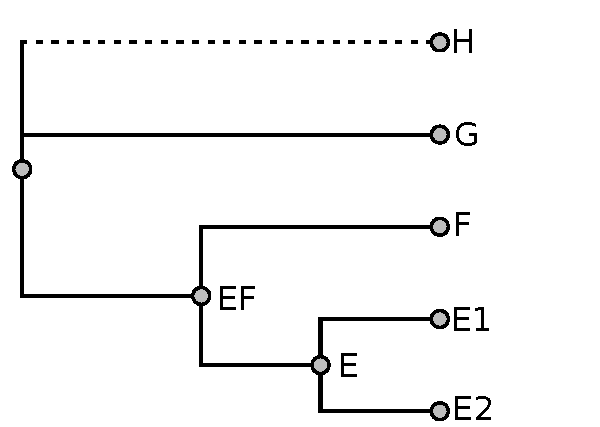
\includegraphics[scale=0.5]{Figures/name1nodes2/tax-shaded}

}\hfill{}\subfloat[Solution tree]{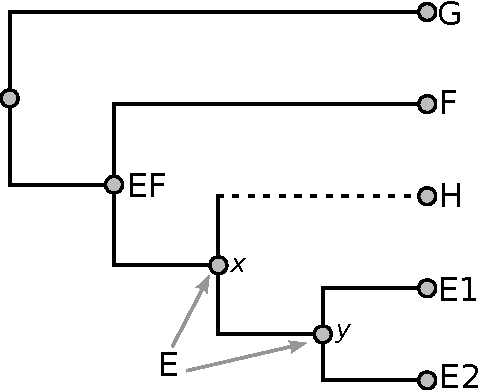
\includegraphics[scale=0.5]{Figures/name1nodes2/solution-shaded}

}\hfill{}

\caption{\label{fig:One-name-can}One name can be consistent with multiple
nodes.}
\end{figure}

It is also possible for multiple names to apply to a single node.
For example, in Figure \ref{fig:Multiple-names-can}a, the taxon $A$
corresponds to the split $B1\,B2\,C\,|\bullet\,Y$, and its child
taxon $B$ corresponds to the split $B1\,B2\,|\bullet\,Y$. The edge
leading to $A$ is consistent with the split for $B$, but the name
$B$ is applied to the node with the smallest include group. However,
in the solution tree (Fig. \ref{fig:Multiple-names-can}b), there
is is only node for both names $A$ and $B$ to apply to. In this
case, we solve this problem by introducing a monotypic parent, and
applying $A$ to the newly created parent node (Fig. \ref{fig:Multiple-names-can}c).
\begin{figure}
\hfill{}\subfloat[Taxonomy tree]{\includegraphics[scale=0.5]{Figures/names2nodes1/tax-shaded}

}\hfill{}\subfloat[Solution tree]{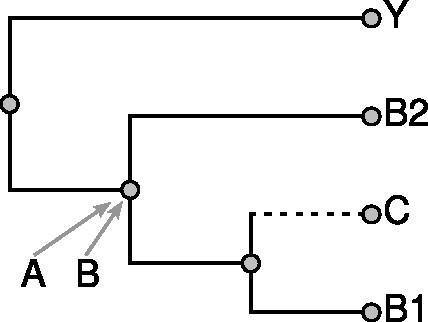
\includegraphics[scale=0.5]{Figures/names2nodes1/synth-shaded}

}\hfill{}\subfloat[Solution tree]{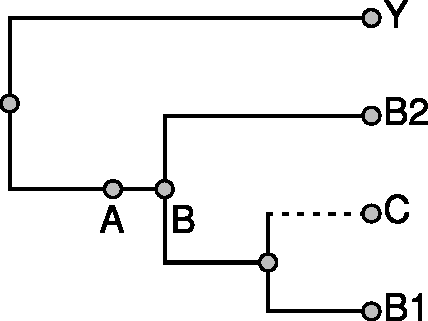
\includegraphics[scale=0.5]{Figures/names2nodes1/solution2-shaded}

}\hfill{}

\caption{\label{fig:Multiple-names-can}Multiple names can apply to a single
node.}

\end{figure}

\emph{}

\subsection{Placement}

After a synthesis tree is constructed, we attach taxon names to the
synthesis tree for each non-conflicting taxon. These names attach
at the MRCA of the include group. Then, for each taxon $A$ that is
found on the synth tree, we associate with the first taxon $B$ found
in a rootward walk on the synthesis tree. If $A$ is not a descendant
of $B$ on the taxonomy, then we say that $A$ is \emph{placed} within
$B$ by the synthesis tree. While this may occur if $A$ is \emph{incertae
sedis}, more complex scenarios are possible. We note that if method
does not handle \emph{incertae sedis} taxa, then this scenario could
not occur because any taxa $B$ that $A$ is placed within would be
considered incompatible with the synthesis tree and so their names
would not be applied.

In order to fully describe a placement of $A$ within $B$ we consider
the sequence of taxa encountered on a walk from $A$ or $B$ up to
their MRCA $M$ on the taxonomy tree. Let us denote the sequence of
taxa encountered from $A$ as $A_{1},\ldots,A_{n},M$ where $A_{1}=A$.
Let $B_{1},\ldots,B_{m},M$ be the sequence of taxa encountered from
$B$ where $B_{1}=B$. Then $A_{n}$ must be \emph{incertae sedis},
and $A_{2},\ldots,A_{n}$ must be incompatible with the synthesis
tree (i.e. broken taxa). We then have that $A$ is placed successively
within $B_{m},B_{m-1},\ldots,B_{2},B_{1}$, and $m$ is the depth
of the placement of $A$.%
\begin{comment}
One question is whether this approach is able to handle nested incertae
sedis taxa.

Placement of incertae sedis taxa by input trees is unfortunately not
quite as simple as finding a single location where an I.S. taxon should
attach. For example, when an incertae sedis taxon is broken, its children
need to be ``placed'' separately.

Each input tree can relate to an \emph{incertae sedis} taxon $(A,B,C)D$
in a number of ways
\begin{itemize}
\item it could resolve $A$, $B$, $C$, or $D$.
\item it could place $D$ on a degree-2 (=out-degree-1) node that bisects
a branch
\item it could place a descendant taxon of $D$ 
\item it could place a descendant taxon of $D$ in a \emph{different place}
than another input tree.
\item it could place children of $D$ in multiple places, thus conflicting
with the branch. If the \emph{incertae sedis} taxon $(A,B,C)$ is
broken, then $A$, $B$ and $C$ become \emph{incertae sedis} clades
in their own right, that may attach separately, except that they .
This is because none of $A$, $B$, or $C$ is in the exclude set
of the siblings of $D$.
\end{itemize}
\end{comment}


\section{Synthesis and conflict resolution with incertae sedis taxa}

\subsection{Placement causes broken taxa}

Synthesis with \emph{incertae sedis} taxa has the potential to resolve
uncertain taxon placements using information from phylogenies. The
propinquity pipeline has always been able to do this kind of resolution.
However, without special consideration given to \emph{naming}, placing
a taxon $A$ within a taxon $B$ results in conflict with taxon $B$
in the taxonomy. In order to avoid a situation where input phylogenies
conflict with a large number of taxa when \emph{incertae sedis} taxa
are placed within them, we have filtered \emph{incertae sedis} taxa
from the taxonomy when constructing all prior synthesis trees.

When the synthesis tree conflicts with a taxonomy node, we way that
the taxon $B$ at that node is a broken taxon. Broken taxa have two
main effects, both of which are negative. First, the name $B$ of
the broken taxon is removed from the synthesis tree. Second, the conflicting
edge for taxon $B$ is not included in the synthesis tree. This means
that any children of $B$ that are taxonomy-only will not be placed
with the children of $B$ that are mentioned in input phylogenies.
Instead the taxonomy-only children of a broken taxon move towards
the root of the synthesis tree and attach at the first higher-ranked
taxon that is an ancestor of $B$ but is not broken.

\subsection{Correctly handling placement}

Thus, we seek a synthesis method that can correctly place taxa within
containing taxa without breaking the containing taxa. We change the
semantics of names to imply, not the exclusion of all non-included
taxa, but only some non-included taxa, as described in section \ref{sec:Semantics-of-incertae}.
As a result of this change in semantics, placing an IS taxon $A$
within a sister taxon $B$ no longer results in conflict with $B$.
This allows us to retain the split for $B$ within the synthesis tree,
so that taxonomy-only children of $B$ are correctly grouped with
their siblings that are referenced by the input trees. We may then
retain the name for the no-longer-broken taxon. Finally, we are then
able to stop filtering \emph{incertae sedis} taxa, so that they appear
in the synthesis tree. Thus, the synthesis tree is able to represent
substantially more species, without suffering the loss of taxa and
the loss of structure.

\subsection{Conflict with incertae sedis taxa}

\subsubsection{Conflicting placement among input trees}

The addition of \emph{incertae sedis} taxa allows new types of conflict
between input trees. For example, different input trees might place
an incertae sedis taxon in conflicting locations. This is illustrated
in Figure \ref{fig:placement-example1}, where the IS taxon (ott7,ott6)ott10
is placed as sister to ott1 by phylogeny $\tau_{1}$ and as sister
ott3 by phylogeny $\tau_{2}$. 

When this happens, the placement of the IS taxon is not influenced
by its being marked IS on the taxonomy. Thus, in Example 1, the higher
ranked tree $\tau_{1}$ will be reflected in the synthesis tree, ott10
will be placed as sister to ott1. In contrast, the conflicting placement
in $\tau_{2}$ will not be reflected in the synth tree. 

All this would occur in the previous version of propinquity. Where
the updated version differs that (a) the names ott9 and ott8 are retained
instead of being dropped. (b) as a result of not breaking ott8 and
ott9, we do not move ott3 and ott2 up to ott11. {[}BDR: Extend more
figures!{]}

\subsubsection{Example B}

However, incertae sedis taxa are not always tip nodes, but may themselves
contain other taxa. In such cases, it is possible for input trees
to conflict with the incertae sedis taxon itself. For example, consider
the following example
\begin{itemize}
\item $T_{1}=((w_{1},w_{2},z_{1}),y_{1})$
\item $T_{2}=((y_{1},y_{2},z_{2}),w_{1})$
\item Taxonomy tree $((w_{1},w_{2})w,(y_{1},y_{2})y,(z_{1},z_{2},z_{3})z)$
with $z$ marked \emph{incertae sedis}.
\begin{itemize}
\item splits $w_{1}w_{2}|\bullet y_{1}y_{2}$, $y_{1}y_{2}|\bullet w_{1}w_{2}$
and $z_{1}z_{2}|\bullet w_{1}w_{2}y_{1}y_{2}$
\end{itemize}
\end{itemize}
In this case, tree $T_{1}$ places $z_{1}$ within $w$, while $T_{2}$
places $z_{2}$ within $y$. Since different members of $z$ are placed,
neither placement for $z$ is rejected. Instead the taxon $z$ is
broken, the name $z$ disappears, and $z_{3}$ floats to the top level. 

Furthermore, since taxon $z$ is a broken \emph{incertae sedis }taxon,
all of its children are effectively incertae sedis independently,
with the difference that they cannot be placed within each other.
Therefore, the names $w$ and $y$ are not lost, since the taxa placed
within them are \emph{incertae sedis} names. Note that $z_{3}$ maybe
therefore be placed in a third location, since it is also \emph{incertae
sedis}.

The situation here would be different if the monophyly of $z$ was
supported by an input phylogeny.

\emph{Note that the synthesis of all input trees before the taxonomy
is unaffected by incertae sedis information.}

\subsubsection{Example C - Nested \emph{incertae sedis} taxa}

In addition to incertae sedis taxa containing other taxa, it is also
possible for incertae sedis taxa to contain nested \emph{incertae
sedis} taxa. \textbf{What issues might this raise?}

\section{Cases}

When only tip nodes on the taxonomy are \emph{incertae sedis}, we
have a very simple form of the \emph{incertae sedis} supertree problem.
However, in practice entire clades may be \emph{incertae sedis}, and
so more complex issue arise. In this section we consider a number
of cases that must be handled when attempting to place \emph{incertae
sedis} taxa.

\subsection{Case 1: An \emph{incertae sedis} clade}

When a clade is marked as \emph{incertae sedis}, we need to consider
two cases. In the first case, the clade may be placed within a sister
clade intact (Figure \ref{fig:Handling-incertae-sedis}). However,
if the clade is not monophyletic in the synthesis tree, then we allow
the members of the clade to be placed separately (Figure \ref{fig:Broken-incertae-sedis}).

\begin{figure}
\subfloat[Input tree \#1]{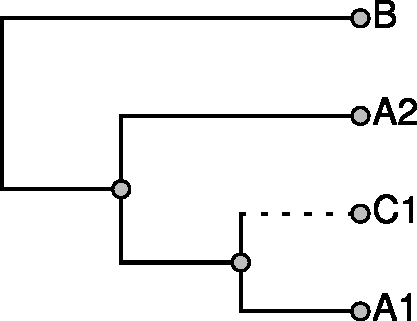
\includegraphics[scale=0.5]{Figures/is-clade/tree1-shaded}

}\hfill{}\subfloat[Taxonomy]{\includegraphics[scale=0.5]{Figures/is-clade/tax-shaded}

}

\subfloat[Synthesis Tree \#1]{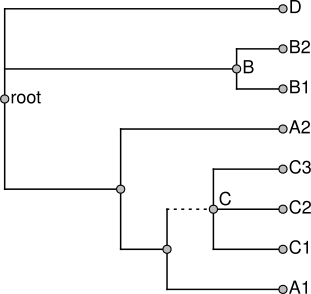
\includegraphics[scale=0.5]{Figures/is-clade/synth1-no-is-shaded}

}\hfill{}\subfloat[Synthesis Tree \#1]{\includegraphics[scale=0.5]{Figures/is-clade/synth1-shaded}

}

\caption{\label{fig:Handling-incertae-sedis}Handling \emph{incertae sedis
}taxa recovers additional edges and taxon names. Supertree construction
on input tree (a) and taxonomy tree (b) with \emph{incertae sedis}
clade $C$ leads to synthesis tree (c). However, supertree construction
with \emph{incertae sedis} handling constructs tree (d), which recovers
taxon name $AB$ and $A$, as well as the edge to clade $AB$. Taxon
names and edges that are conditional on handling \emph{incertae sedis}
are shaded grey. }

\end{figure}

\begin{figure}

\hfill{}\subfloat[Input tree \#1]{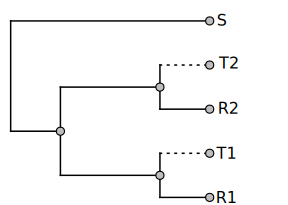
\includegraphics[scale=0.5]{Figures/is-clade/tree2-shaded}

}\hfill{}\subfloat[Taxonomy]{\includegraphics[scale=0.5]{Figures/is-clade/tax-shaded}

}\hfill{}

\hfill{}\subfloat[Synthesis Tree \#1]{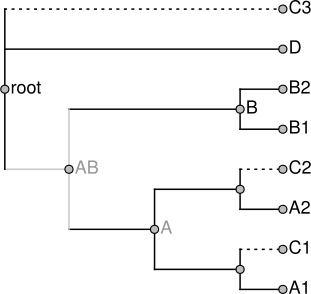
\includegraphics[scale=0.5]{Figures/is-clade/synth2-shaded}

}\hfill{}

\caption{Broken incertae sedis clade\label{fig:Broken-incertae-sedis}. Taxonomy
tree (b) contains \emph{incertae sedis }taxon $C$ that is broken
by input tree (a). Supertree construction results in a synthesis tree
(c) that places $C1$ and $C2$ separately within $A$.}

\end{figure}


\subsection{Case 2: A nested \emph{incertae sedis} clade}

When \emph{incertae sedis} clades are allowed, it is possible for
an \emph{incertae sedis} taxon to be nested within another \emph{incertae
sedis} taxon. In such a case we must allow the higher-ranked taxon
to be placed within a sibling, while preserving the right of the lower
ranked taxon to be placed within a lower-level sibling (Figure \ref{fig:Nested-incertae-sedis}).

\begin{figure}
\subfloat[Input tree \#1]{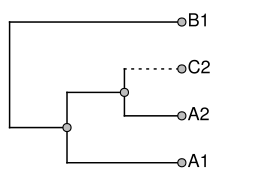
\includegraphics[scale=0.5]{Figures/is-nested/tree3-shaded}

}\hfill{}\subfloat[Taxonomy tree]{\includegraphics[scale=0.5]{Figures/is-nested/tax-shaded}

}

\subfloat[Synthesis tree (\emph{incertae sedis} ignored)]{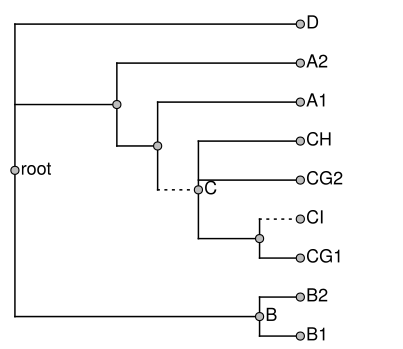
\includegraphics[scale=0.5]{Figures/is-nested/synth3-no-is-shaded}

}\hfill{}\subfloat[Synthesis tree (\emph{incertae sedis} considered)]{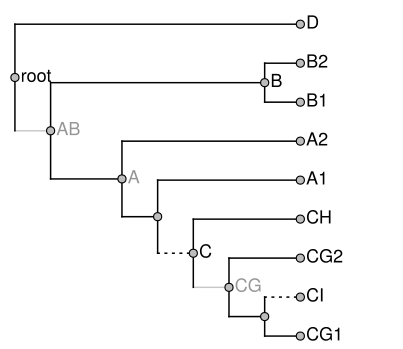
\includegraphics[scale=0.5]{Figures/is-nested/synth3-is-shaded}

}

\caption{\label{fig:Nested-incertae-sedis}Nested incertae sedis taxa. (a)
Input tree \#1 places CI1 within CG, and C within $A$. (b) In the
taxonomy, CI is \emph{incertae sedis }within C, while C is \emph{incertae
sedis} under the root. (c) The synthesis tree when \emph{incertae
sedis} taxa are not considered. The names AB, A, and CG are lost.
(d) The synthesis tree when \emph{incertae sedis} taxa are considered.
The names AB, A, and CG are regained, as well as the edges leading
to AB and CG.}

\end{figure}


\subsection{Case 3: Placement of one incertae sedis taxon within another.}

In our semantics of incertae sedis taxa, it is possible for to place
one \emph{incertae sedis} sibling inside another. A special case of
this is when a higher-rank incertae sedis taxon $A$ is placed as
sister to an incertae sedis taxon $B$, and then $B$ is placed within
$A$ (Figure \#).

\emph{This case makes placement more complicated. Use a sequence of
ordered placements, preorder?}
\begin{figure}

\subfloat[Input tree \#1]{\includegraphics[scale=0.5]{Figures/is-within-is/tree1\lyxdot tre}

}\subfloat[Taxonomy]{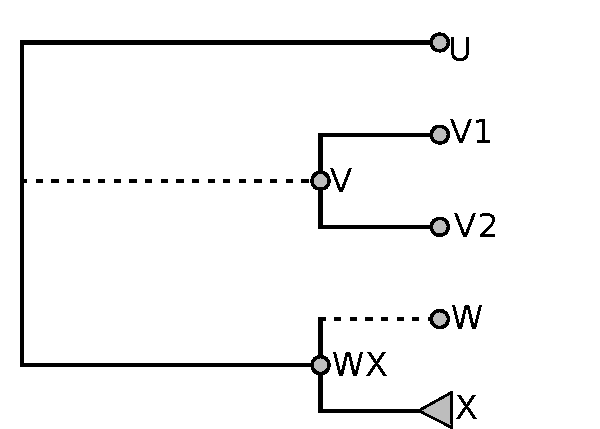
\includegraphics[scale=0.5]{Figures/is-within-is/tax-shaded}

}\subfloat[Synthesis tree]{\includegraphics[scale=0.5]{Figures/is-within-is/synth1-shaded}

}

\caption{Placing one incertae sedis group within another. Here I is placed
within A, and then AI is placed within A.}

\end{figure}


\section{Handling \emph{incertae sedis} taxa in the propinquity pipeline}

In order to handle \emph{incertae sedis} taxa within propinquity,
we must modify some of the stages of the propinquity pipeline. Subproblem
decomposition must place \emph{incertae sedis} taxa in the correct
subproblem. Subproblem files must indicate which taxa are incertae
sedis. The subproblem solver must read this information, account for
\emph{incertae sedis} taxa when solving subproblems, and correctly
name taxa that have been modified by having \emph{incertae sedis}
taxa place inside them. The unpruner must be aware of \emph{incertae
sedis} taxa. Annotations of the tree must be aware of \emph{incertae
sedis} taxa so that it does not consider taxa broken when they have
an incertae sedis taxon placed inside them.

\subsection{Exemplifying taxa}

One current problem is that well-known taxa like Fungi or Mammalia
tend to have a very large number of incertae sedis children, making
browsing in the tree viewer difficult. This can happen when, for example,
fossils or other hard-to-place taxa get classified only to the level
of these well-known nodes and no further. This leads to a situation
where well-known taxa serve as a dumping ground for unplaced taxa.

Our current approach to this problem is to perform a second round
of pruning, or ``cleaning'', during the exemplification step. Incertae
sedis taxa are pruned at this stage if they do not occur in any input
trees. We thus generate a second ``cleaned taxonomy'' that has undergone
this further round of cleaning. This approach improves on the previous
approach in that \emph{incertae sedis} taxa in input trees are no
longer pruned. This approach also removes tons of \emph{incertae sedis}
children from nodes like ``Fungi'', where a lot of unplaced fossils
with few observable characters have been dumped. 

However, this approach has the negative effect of pruning some incertae
sedis taxa that need not be pruned. For example, suppose \emph{incertae
sedis} taxon $A$ contains 5 children, of which only 1 child $A_{1}$
occurs in an input tree. If the taxon $A$ is not broken, then it
should be possible to attach the other 4 members of $A$ next to $A_{1}$,
without cluttering up the synthesis tree. Such taxa have been successfully
placed even though they are not in any input tree. This can only be
discovered after synthesis is complete, though.

Additionally, it should also be possible to filter unplaced taxa in
the tree viewer instead of in the synthesis pipeline.

\subsection{Sub-problem decomposition}

The presence of \emph{incertae sedis }taxa poses a problem to sub-problem
decomposition, since taxonomy edges no longer completely separate
subproblems. Instead, \emph{incertae sedis} taxa may attach on either
side of a taxonomy edge. We seek to place \emph{incertae sedis} taxa
into subproblems in such a way that the subproblem solver can perform
the placement inside the subproblem. This approach postpones handling
of conflict in \emph{incertae sedis} taxa to the subproblem solver,
where the problem is well formulated in terms of splits. However,
it does have the effect of creating larger subproblems.

We must also handle conflicting placements of \emph{incertae sedis}
taxa by different input trees. Thus, if one input tree places the
\emph{incertae sedis} taxon $X$ in $((X)B)A$ and another places
$X$ in $((X)C)A$ then we must mark both edges $B$ and $C$ as contested
edges, even if these edges would \emph{not} be contested were taxon
$X$ to be removed. This results in a new way to contest edges that
involves the interaction of two input trees, and not just the interaction
of each input tree with the taxonomy.

We choose to solve these problems by merging any subproblems that
an \emph{incertae sedis} taxon might be placed in. The simplest way
to achieve this is simply to regard any taxon that has an \emph{incertae
sedis }taxon placed within it as contested. This results in marking
both $B$ and $C$ as contested edges in the example above. In fact,
this is the current behaviour of the non-\emph{incertae-sedis} aware
subproblem decomposer. One downside of this approach is that, if we
have $((X)B)A)$ in one input tree, and $X$ is mentioned nowhere
else, then by marking $B$ as contested, we are merging subproblems
unnecessarily. We could instead placed $X$ in $B$ and avoid contesting
the edge $B$. However, this approach is more complex and does not
seem necessary in practice.

\begin{figure}
\subfloat[Taxonomy $\protect\taxonomy$]{\includegraphics[scale=0.5]{Figures/placement1/tax\lyxdot tre}

}\subfloat[$\tau_{1}$]{\includegraphics[scale=0.5]{Figures/placement1/input1\lyxdot tre}

}\subfloat[$\tau_{2}$]{\includegraphics[scale=0.5]{Figures/placement1/input2\lyxdot tre}

}

\caption{\label{fig:placement-example1}Example. An incertae sedis clade (ott6,ott7)
is placed in different subtrees by input trees $\tau_{1}$ and $\tau_{2}$.
In $\tau_{1}$, two nodes that correspond to the taxonomy their ingroup
extended to include (ott6,ott7), and the branches leading to these
nodes have been colored blue. The dashed blue edge leads to a node
that is a newly-introduced degree-2 node which does not correspond
to any taxonomy node. In $\tau_{2}$, only one node that corresponds
to a taxonomy node needs to have its ingroup extended. The placement
of (ott6,ott7) into ott8 toward ott1 by $\tau_{1}$ conflicts with
the placement of (ott6,ott7) into ott9 toward ott3 by $\tau_{2},$}
\end{figure}
 For example, in Figure \ref{fig:placement-example1}, input tree
$\tau_{1}$ contests ott9 and input tree $\tau_{2}$ contests ott9
and ott8. Thus ott1, ott2, ott3, ott6, and ott7 end up in the same
sub-problem.

\subsection{Subproblem solution}

Our sub-problem solver naturally handles \emph{incertae sedis} taxa.
This is because we define the semantics of \emph{incertae sedis} taxa
in terms of partial splits, and our solver natively supports building
trees from partial splits through its use of the BUILD algorithm.
Handling \emph{incertae sedis} taxa thus requires loading incertae
sedis information and computing partial splits for \emph{incertae
sedis} taxa before solving a sub-problem. After solving a sub-problem,
we must apply taxon names from the taxonomy tree to the sub-problem
solution tree. The solution tree is considered to a fixed tree and
not to have any \emph{incertae sedis} nodes, or any other forms of
uncertainty.

\subsubsection{Reading incertae sedis information}

Currently, we read the \emph{incertae sedis} information as a list
of OTT ids for \emph{incertae sedis} taxa. This does not require adding
further annotations to the node names. Only taxonomy nodes can be
\emph{incertae sedis} at the moment, and only the taxonomy tree for
the subproblem contains OTT ids for internal nodes. Therefore we handle
\emph{incertae sedis} information by constructing modified split sets
for the lowest-ranked tree when the list of \emph{incertae sedis}
nodes is not empty.

\subsubsection{Exclude sets modified by \emph{incertae sedis} marks}

Equation (\ref{eq:exclude-set-formula-1}) leads to the following
algorithm to compute the exclude set for all nodes in a tree.
\begin{enumerate}
\item Set the exclude set of the root node to be empty
\item For each \emph{node} (except the root) in preorder
\begin{itemize}
\item combine the \emph{exclude} set of the parent node with the \emph{include}
set of non-\emph{incertae-sedis} siblings.
\item store this set in a hash, with key \emph{node}
\end{itemize}
\end{enumerate}
This algorithm is currently implemented in \emph{otc-solve-subproblem}.
We store the sets as \emph{std::set}.

\subsubsection{Implementation: finding the node for a name}

To find the node for a name $n$, we find the MRCA of the cluster
$S_{1}(n)$. If the MRCA excludes the entire exclude group $S_{2}(n)$
then the name applies to the MRCA; otherwise the taxon does not exist
on the tree.

\subsubsection{Implementation: handling name clashes}

When multiple names $N=\{n_{1},\ldots n_{N}\}$ map to the same solution
node $x$, then these names must satisfy some tree structure on the
taxonomy, such that $n_{1}<n_{2}$ if $n_{1}$ is a descendant of
$n_{2}$ in the taxonomy. If it is possible to find a name $n_{max}$
that is the unique maximal element of $N$, then it is permissible
to 
\begin{enumerate}
\item create a monotypic parent $p(x)$ of $x$, and assign $n_{max}$ to
$p(x)$
\item continue handling name clashes at $x$ with the set of possible names
reduced to $N-n_{max}$.
\end{enumerate}
However, its certainly possible that there might not be any such $N_{max}$,
in which case we could just choose a name for $x$ from $N$ (perhaps
not an \emph{incertae sedis} name) and then record all the other names
as equivalents somewhere.

\textbf{BDR:}\textbf{\emph{ }}\emph{we might get this behavior in
a nice an automatic way if we create a single fake leaf for each monotypic
taxonomy node that holds the node's leaf label.}

\subsubsection{Caveats}

When multiple I.S. taxa have been moved to the root node of a subproblem,
they may be I.S. over the entire subproblem, and some may be I.S.
over others in an asymmetric manner. Therefore, we might need to specify
additional information about the original attachment location of the
I.S. taxa, such as their depth. This only affects problems that have
been decomposed.

\textbf{BDR:} \emph{currently we don't actually move taxa to get them
into a subproblem. So, is this even an issue?}

\subsection{Grafted supertree}

\emph{Question:} Does the synthesis tree contain any \emph{incertae
sedis} groups?\\
\emph{Answer:} The grafted supertree will not contain any \emph{incertae
sedis} groups. However, when we attach pruned nodes to a parent in
the grafted supertree, we could mark such nodes \emph{incertae sedis}
if we want.

\subsection{Unpruning}

Currently the unpruner \emph{does not} require that the OTT ids are
named in the grafted solution before unpruning starts. According to
Mark's document, he wasn't sure if such names were generated for nodes
that had an IS taxon placed inside of them, so otc-unprune-solution-and-name-unnamed
nodes throws away all the names and generates them itself.

\textbf{BDR}: See document \texttt{otcetera/doc/unprune-solution-and-name-unnamed-nodes.pdf}

The unpruner should record when unpruned nodes are \emph{incertae
sedis}. Such nodes are unaffected by phylogenies, and so \emph{incertae
sedis} annotations for them make good sense.

\subsection{Annotation}

Annotation primarily involves running a conflict analysis between
the synthesis tree and each input tree. Since neither tree has any
\emph{incertae sedis} taxa, the conflict algorithm does not need to
change. Furthermore, if we allow \emph{incertae sedis} taxa that are
taxonomy-only to be annotated as \emph{incertae sedis} on the synth
tree, then such groups will not affect conflict with the input trees.
We would also like to allow running a conflict analysis between the
synthesis tree and the taxonomy tree. However, naming the nodes \emph{is}
a (almost) run of conflict analysis on the taxonomy tree, and this
has already been done in a prior step. So, the current annotation
procedure actually works as-is.

It would be nice to allow running conflict against the cleaned taxonomy,
though. One way to do this would be to generated a ``placed taxonomy'',
with groups extended to include \emph{incertae sedis} taxa that have
been placed within them. This would not require any updating to the
conflict-analysis code in the annotation step.

\subsection{Conflict service}

The current conflict service considers a group $A$ to conflict with
the taxonomy if group $A$ has an incertae sedis group $B$ placed
within it. This doesn't affect the annotations, since taxon names
are added by the unpruner. But it could make perfectly fine input
trees incorrectly look like they are the cause of broken taxa, if
they contain IS taxa. Thus, it would be nice to have a modified conflict
algorithm. 

\subsubsection{Current conflict algorithm}

The current conflict algorithm is pretty fast, but it works by classifying
tips into either (i) the include group or (ii) the exclude group.
To avoid counting the exclude group for every split, we instead count
the total number of children for each node, and assume that any children
not in the include set are in the exclude set. This is no longer true
when we have incertae sedis taxa. I suspect that if we want to handle
incertae sedies, we'd need a third category (iii) for ``neither include
group nor exclude group''.
\begin{enumerate}
\item Get induced trees on intersection of leaf sets
\item Compute depth for each node (nd->depth)
\item Compute number of tips at or below each node (nd->n\_tips)
\item for each input tree node -> $nd$
\begin{enumerate}
\item skip the root
\item skip monotypic
\item if its a tip then find corresponding (``terminal'') edges in synth
tree and continue
\item leaves1 <- get the list of leaves in the include group of $nd$ (in
input)
\item L2 <- find the total number of tips (L2 = sum {[}nd->n\_tips| nd <-
leaves1{]})
\item leaves2 <- get list of corresponding synth leaf nodes (in synth)
\item nodes <- find all nodes between leaves2 and the MRCA (in synth)
\item MRCA <- mrca of leaves2 (in synth. this uses the nd->depth annotation)
\item Compute number of tips in the include set (nd->include\_tips) below
each node in $nodes$ (in synth)
\item if n\_include\_tips(MRCA) == n\_tips(MRCA) then the MRCA displays
$nd$
\item if n\_include\_tips(MRCA) < n\_tips(MRCA) then
\begin{itemize}
\item foreach node in nodes
\begin{itemize}
\item if (n\_include\_tipes(nd) < n\_tips(nd) and n\_include\_tips(nd) <
l2)
\begin{itemize}
\item this is a conflict!
\end{itemize}
\end{itemize}
\item if there are no conflicts, then this is a resolved\_by.
\end{itemize}
\end{enumerate}
\end{enumerate}

\subsubsection{Modified conflict algorithm?}

This probably is outside the scope of the paper, but if we could come
up with a modified conflict algorithm, that would be nice/useful,
and probably novel. It would also probably be slower...

\section{Results}

\subsection{Case 1}

taxonomy = (((a1,a2)A,(b1,b2)B)AB,(c1,c2)?C,D)root;

\subsubsection{If we place $c$ within $A$}

tree1 = (((a1,c1),b1),d1);

synth-with-is: ((((a1,(c1,c2)C),a2)A,(b1,b2)B)AB),(d1)D)

placement: C within A <- AB 

synth-no-is: ((a1,(c1,c2)C),a1,(b1,b2)B,(d1)D)

\subsubsection{If we place $c$ within $A$ but break $C$}

tree1 = ((a1,c1),(a2,c1),b1)

synth-with-is: ((((a1,c1),(a2,c2))A,(b1,b2)B)AB, (d1)D)

synth-no-is: ??

placement: 
\begin{itemize}
\item c1 <- (broken) C within A <- AB.
\item c2<- (broken) C within A <- AB
\end{itemize}
result: we lose $C$, but keep $A$ and $AB$.

\subsection{Case 2: nested is}

taxonomy = (((a1,a2)A,(b1,b2)B),( ( (c11,c12)C1,(c21,c22)C2,(ci1,ci2)?CI
)?C) ,(d1)D)

tree1 = ((a1,(c11,(ci1,c12))),b1)

synth-with-is: places CI wihin C1, and C within A.

\subsection{Case 3: interleaving taxa}

taxonomy = ((a1,a2)A,(b1,b2)?B,(c1,c2)?c)

input tree: ((b1,c1),(b2,c2))

synth-with-is: ((a1,a2)A,((b1,c1),(b2,c2))B) or ((a1,a2)A,((b1,c1),(b2,c2))C)

Result: we name the interleaved taxon $B$ or $C$, but cannot name
it both names.

\subsection{Case 4: creation of monotypic taxa}

see test cases.
\begin{lyxcode}
\begin{comment}
\begin{lyxcode}
\textbf{Whale:}~?ott6145835~{[}6145835~Brandtocetus/genus{]}~<-~ott698424~{[}698424~Cetacea/order{]}~placed~under~ott4942423~{[}4942423~Cetotherium~/~genus{]}~<-~ott698424~{[}698424~Cetacea/order{]}

\textbf{Whale:}~?ott6145873~{[}6145873{]}~<-~ott698424~{[}698424~Cetacea~/~order{]}~placed~under~ott4942423~{[}4942423{]}~<-~ott698424~{[}698424{]}~

-~Cetacea~broken.

\textbf{Insect:}~?ott18090~{[}18090{]}~<-~ott672501~{[}672501{]}~placed~under~ott275501~{[}275501{]}~<-~ott672501~{[}672501{]}

\textbf{Insect:}~?ott190269~{[}190269{]}~<-~ott672501~{[}672501{]}~placed~under~ott275501~{[}275501{]}~<-~ott672501~{[}672501{]}~

\textbf{Insect:}~?ott349638~{[}349638{]}~<-~ott672501~{[}672501{]}~placed~under~ott275501~{[}275501{]}~<-~ott672501~{[}672501{]}~

\textbf{Insect:}~?ott1009313~{[}1009313{]}~<-~ott672501~{[}672501~Reduviidae~/~family{]}~placed~under~ott275501~{[}275501{]}~<-~ott672501~{[}672501{]}~

-~Reduviidae~broken.

\textbf{Insect:~}?ott564110~{[}564110{]}~<-~ott939130~{[}939130~Thyrididae~/~family{]}~placed~under~ott757344~{[}757344{]}~<-~ott939130~{[}939130{]}~

\textbf{Plant:}~?ott679485~{[}679485{]}~<-~ott1074933~{[}1074933~Lamioidea~/~subfamily{]}~placed~under~ott534796~{[}534796{]}~<-~

\textbf{Plant:}~?ott729184~{[}729184{]}~<-~ott1074933~{[}1074933~Lamioidea~/~subfamily~{]}~placed~under~ott534796~{[}534796{]}~<-~ott1074933~{[}1074933{]}~

ott1074933~{[}1074933{]}~

-~Lamioidea~\emph{not}~broken

\textbf{Plant:}~?ott5144555~{[}5144555{]}~<-~ott23373~{[}23373{]}~placed~under~ott447802~{[}447802{]}~<-~ott23373~{[}23373{]}

-~Orobanchaceae~broken

\textbf{Fly:}~?ott441413~{[}441413~Rhodesiella~lungliensis/species{]}~<-~ott1014022~{[}1014022~Rubiaceae{]}~placed~under~ott571842~{[}571842~Pavetteae~/~tribe{]}~<-~ott997381~{[}997381~Ixoroidea/subfamily{]}~<-~ott1014022~{[}1014022~Rubiaceae/family{]}

\textbf{Plant:}~?ott31033~{[}31033{]}~<-~ott627035~{[}627035{]}~placed~under~ott6019314~{[}6019314{]}~<-~ott627035~{[}627035{]}~

\textbf{Bacteria:}~?ott4018918~{[}4018918{]}~<-~ott5248084~{[}5248084{]}~placed~under~ott167767~{[}167767{]}~<-~ott5248084~{[}5248084{]}~

\textbf{Bacteria:}?ott4792759~{[}4792759{]}~<-~ott5248084~{[}5248084{]}~placed~under~ott167767~{[}167767{]}~<-~ott5248084~{[}5248084{]}~

-~Erysipelotrichaceae~broken
\end{lyxcode}
\end{comment}
\end{lyxcode}
Should we do this? We could say: 
\begin{itemize}
\item there are 331 incertae sedis taxa that are mentioned in input trees.
\begin{itemize}
\item what is the kingom / phylum / class / order / genus / species
\end{itemize}
\item we placed 14 incertae sedis taxa inside a sister taxon. (``incertae
sedis'', ``versus ``unplaced''?)
\item we placed $o$ incertae sedis taxa \emph{outside} all sister taxa.
\item we confirmed $n$ incertae sedis taxa as being separate from all sister
(sampled) taxa??
\item we avoiding breaking 8 taxa that had IS taxa placed inside them.
\item we allowed $z_{1}$ new taxa into the synthesis tree that were incertae
sedis.
\item we allowed $z_{2}$ new taxa into the synthesis tree that are marked
as extinct.
\item some nodes have as many as $w$\emph{ incertae sedis} children, making
them unbrowseable when incertae sedis children are not excluded.
\item $v_{1}$ input trees were previously excluded \emph{entirely} because
they are nested within in an incertae sedis taxon.
\item $v_{2}$ input trees were previously excluded \emph{partially} because
they are nested within in an incertae sedis taxon.
\end{itemize}
Currently the numbers $z_{1}$ and $z_{2}$. 

\section{Discussion}

One thing we could do (perhaps) that we are not currently doing, is
to have nodes marked as incertae sedis on the synth tree. This would
be easy enough if such nodes are not affected in any way by the input
trees. Thus, when unpruning nodes we could mark any nodes \emph{incertae
sedis} if they were marked \emph{incertae sedis} on the taxonomy.

Secondly, I think we need to distinguish \emph{incertae sedis} taxa
that are ``unplaced'' from \emph{incertae sedis} taxa that do not
occur in any input tree. I think that if $A$ contains child $A_{1}$
that is an input tree, and the taxon $A$ is not broken, then $A$
will be placed, and thus any other children $A_{2},A_{3},\ldots,A_{n}$
will also be placed, since they will be added as children of the (placed)
node $A$ by the unpruner. This could be considered when deciding
which nodes to suppress in the tree viewer.

\paragraph{Taxonomy merging}

Not all \emph{incertae sedis} taxa in our taxonomy are directly labeled
\emph{incertae sedis} by taxonomists. \emph{Incertae sedis} taxa can
also result from automatic merging of taxonomies to create the OpenTree
taxonomy. For example, in Figure 3 of \citet{rees2017automated},
cases \#4 and \#6 illustrate examples where merging of two taxonomies
leads to a taxonomy with a taxon of uncertain placement. The reason
is primarily that if taxonomy $\taxonomy_{1}$ contains more levels
of hierarchy than taxonomy $\taxonomy_{2}$, then we must add internal
nodes to $\taxonomy_{2}$ to align it to $\taxonomy_{1}$. However,
if taxonomy $\taxonomy_{2}$ contains more leaves than $\taxonomy_{1}$,
then it is unclear if these extra leaves should be nested inside the
additional internal nodes, or not. Thus, the extra leaves are marked
\emph{incertae sedis}.

For example, if $\taxonomy_{1}=((a,b)x,(c,d)y)z$ and $\taxonomy_{2}=(a,b,c,d,e)z$
then $a$ and $b$ in $\taxonomy_{2}$ should be nested within $x$,
but we do not know if $e$ should be nested within $x$ or not. Thus
we obtain $((a,b)x,(c,d)y,?e)z$, where $?$ indicates that taxon
$e$ is marked \emph{incertae sedis}.

If incertae sedis taxa are cannot be placed within other incertae
sedis taxa, then such an approach does not work if $y$ is already
incertae sedis. However, we take the approach that \emph{incertae
sedis} notations are not a general solution to expression of uncertain
placement.

\subsubsection{Comparison to operational definition}

The splits-based semantics for incertae sedis taxa has many desirable
properties. In allows the use of the BUILD algorithm to assess compatibility
of split sets. However, it also has some properties that may not be
expected. For example, two incertae sedis siblings can be freely interdigitated,
which might not be the expected outcome. The current definition, also
ignore ranks. Thus if we had two incertae sedis siblings that were
genera, but other siblings were families, then one might expect that
the genus-level incertae sedis taxa could be placed within families,
but not intermixed. Since the current approach ignores ranks, it cannot
do that.

The above definition of incertae sedis taxa does allow two incertae
sedis sister taxa to be interdigitated. It also 

Also, the splits-based semantics might not completely recover the
edit-operation semantics. The corner cases are ... .

\subsubsection{Intrusion into incertae sedis taxa}

In theory it could be possible for an \emph{incertae sedis} taxon
$A$ to be placed within an \emph{incertae sedis} sibling $B$. We
initially implemented this semantics. It requires updating the recursion
to define $I(m,n)$ as the descendants of $m$ that can be access
from $n$ without traversing an \emph{incertae sedis} node.

With a splits-based semantics, we cannot allow both (i) placing $A$
in $B$ and (ii) placing $B$ in $A$ and also forbid interdigitating
$A$ and $B$.

However, if we allow this behavior by reducing the exclude sets for
$A$ and $B$, then this has the unfortunate consequence that the
members of $A$ and $B$ may be inter-digitated. In many cases, \emph{incertae
sedis} genera have siblings that are families, and the expected semantics
is that genera may be placed within their sibling families, or may
remain outside existing families. In such cases, inter-digitating
the genera would not be expected behavior. Thus, we choose the semantics
that \emph{incertae sedis} taxa exclude their \emph{incertae sedis}
siblings. This is not because the other semantics is impossible. However,
we note that use of the interdigitating semantics allows a situation
where the names for $A$ and $B$ both apply to the same node.

This semantics also complicates placement, since it is possible to
place $A$ as a sibling of $B$, and then place $B$ within $A$.
This violates the current invariant that taxa are only ever placed
within more tipward taxa. This makes the description of placement
more complicated, since we can no longer simply record all cases where
a parent node is not ancestor on the taxonomy.

\subsubsection{Usage in the literature}

The term \emph{incertae sedis} can be used in a number of different
ways. For example,\emph{ }one author might describe \emph{incertae
sedis} genera that are asserted to be monophyletic, whereas another
author might describe \emph{incertae sedis} genera that may be interdigitated. 

\bibliographystyle{upmplainnat}
\bibliography{otcetera}

\end{document}
